\item As shown in the figure, a combination of a thin plano concave lens and a thin plano convex lens is used to image an object placed at infinity. The radius of curvature of both the lenses is 30cm and refraction index of the material for both the lenses is 1.75. Both the lenses are placed at distance of 40cm from each other. Due to the combination, the image of the object is formed at distance x = \underline{\hspace{2.5cm}} cm, from concave lens.
    \begin{center}
        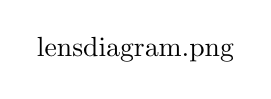
\begin{tikzpicture}
            \node at (0, 0) {{lensdiagram.png}};
        \end{tikzpicture}
    \end{center}